\documentclass{standalone}
\usepackage{tikz}
\usetikzlibrary{patterns, positioning}


\begin{document}
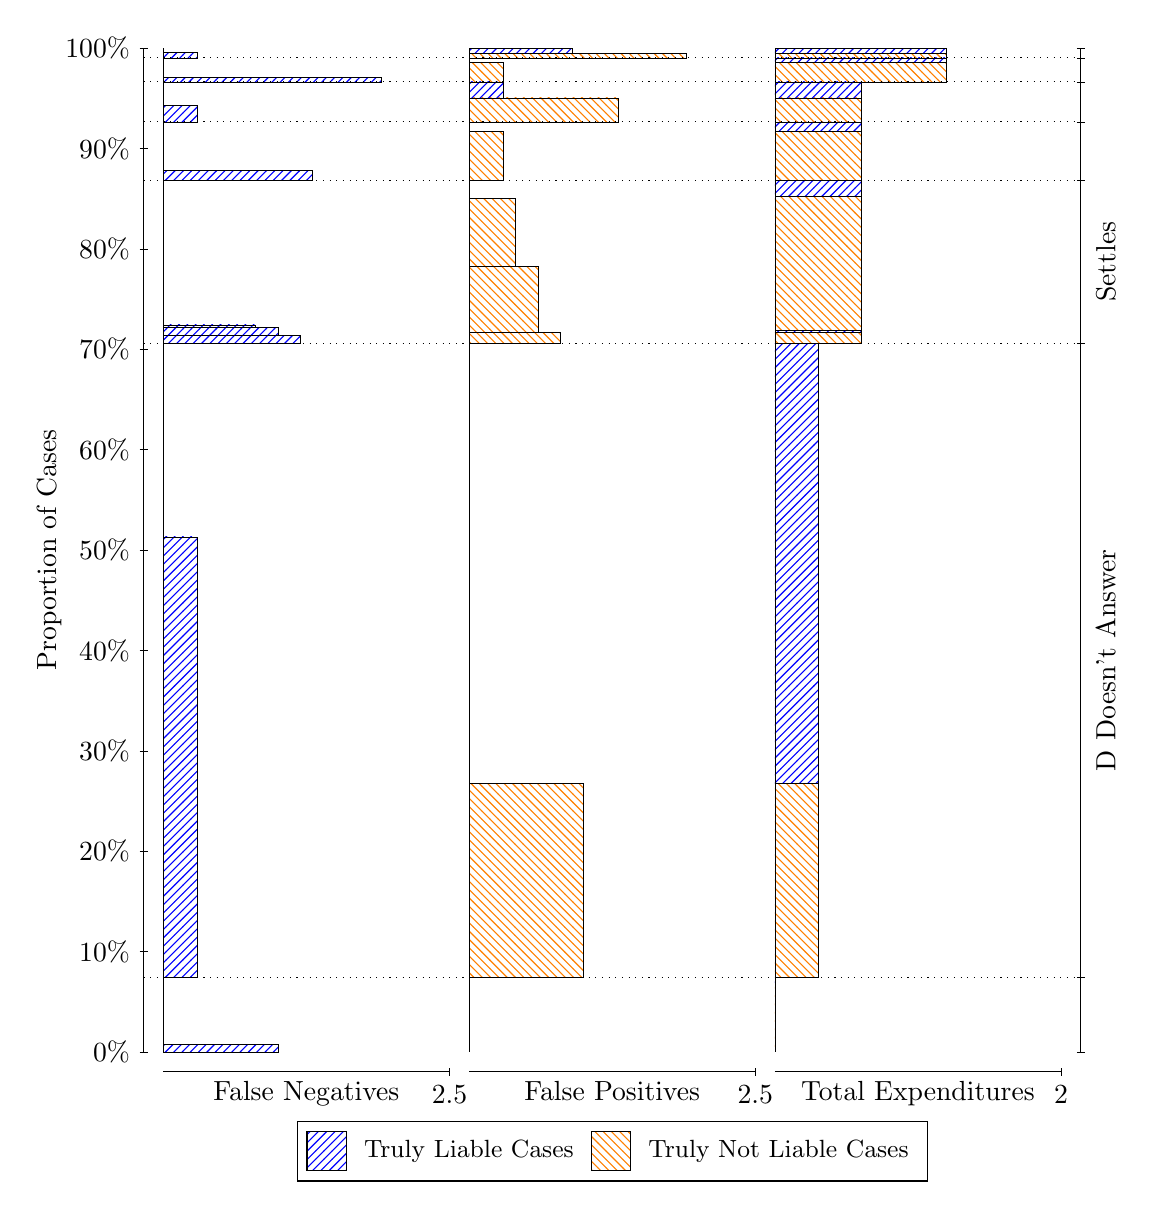
\begin{tikzpicture}
\draw[black, very thin] (1.5,1.75) -- (1.5,14.5);
\node[rotate=90, text=black, anchor=center] at (0.3, 8.125) {Proportion of Cases};
\draw[black, very thin] (1.45,1.75) -- (1.55,1.75);
\node[text=black, anchor=east] at (1.45, 1.75) {0\%};
\draw[black, very thin] (1.45,3.025) -- (1.55,3.025);
\node[text=black, anchor=east] at (1.45, 3.025) {10\%};
\draw[black, very thin] (1.45,4.3) -- (1.55,4.3);
\node[text=black, anchor=east] at (1.45, 4.3) {20\%};
\draw[black, very thin] (1.45,5.575) -- (1.55,5.575);
\node[text=black, anchor=east] at (1.45, 5.575) {30\%};
\draw[black, very thin] (1.45,6.85) -- (1.55,6.85);
\node[text=black, anchor=east] at (1.45, 6.85) {40\%};
\draw[black, very thin] (1.45,8.125) -- (1.55,8.125);
\node[text=black, anchor=east] at (1.45, 8.125) {50\%};
\draw[black, very thin] (1.45,9.4) -- (1.55,9.4);
\node[text=black, anchor=east] at (1.45, 9.4) {60\%};
\draw[black, very thin] (1.45,10.675) -- (1.55,10.675);
\node[text=black, anchor=east] at (1.45, 10.675) {70\%};
\draw[black, very thin] (1.45,11.95) -- (1.55,11.95);
\node[text=black, anchor=east] at (1.45, 11.95) {80\%};
\draw[black, very thin] (1.45,13.225) -- (1.55,13.225);
\node[text=black, anchor=east] at (1.45, 13.225) {90\%};
\draw[black, very thin] (1.45,14.5) -- (1.55,14.5);
\node[text=black, anchor=east] at (1.45, 14.5) {100\%};

\draw[black, very thin] (13.4,1.75) -- (13.4,14.5);
\draw[black, very thin] (13.35,1.75) -- (13.45,1.75);
\node[anchor=west] at (13.35, 1.75) {};
\draw[black, very thin] (13.35,2.699) -- (13.45,2.699);
\node[anchor=west] at (13.35, 2.699) {};
\draw[black, very thin] (13.35,10.753) -- (13.45,10.753);
\node[anchor=west] at (13.35, 10.753) {};
\draw[black, very thin] (13.35,12.82) -- (13.45,12.82);
\node[anchor=west] at (13.35, 12.82) {};
\draw[black, very thin] (13.35,13.562) -- (13.45,13.562);
\node[anchor=west] at (13.35, 13.562) {};
\draw[black, very thin] (13.35,14.071) -- (13.45,14.071);
\node[anchor=west] at (13.35, 14.071) {};
\draw[black, very thin] (13.35,14.376) -- (13.45,14.376);
\node[anchor=west] at (13.35, 14.376) {};
\draw[black, very thin] (13.35,14.5) -- (13.45,14.5);
\node[anchor=west] at (13.35, 14.5) {};

\draw[black, very thin, pattern color=blue, pattern=north east lines] (1.75,1.75) rectangle (3.2033,1.8498);
\draw[black, very thin, pattern color=orange, pattern=north west lines] (1.75,1.8498) rectangle (1.75,2.699);
\draw[black, very thin, pattern color=blue, pattern=north east lines] (1.75,2.699) rectangle (2.186,8.2915);
\draw[black, very thin, pattern color=orange, pattern=north west lines] (1.75,8.2915) rectangle (1.75,10.753);
\draw[black, very thin, pattern color=blue, pattern=north east lines] (1.75,10.753) rectangle (3.494,10.85);
\draw[black, very thin, pattern color=blue, pattern=north east lines] (1.75,10.85) rectangle (3.2033,10.953);
\draw[black, very thin, pattern color=blue, pattern=north east lines] (1.75,10.953) rectangle (2.9127,10.983);
\draw[black, very thin, pattern color=orange, pattern=north west lines] (1.75,10.983) rectangle (1.75,12.82);
\draw[black, very thin, pattern color=blue, pattern=north east lines] (1.75,12.82) rectangle (3.6393,12.942);
\draw[black, very thin, pattern color=orange, pattern=north west lines] (1.75,12.942) rectangle (1.75,13.562);
\draw[black, very thin, pattern color=blue, pattern=north east lines] (1.75,13.562) rectangle (2.186,13.767);
\draw[black, very thin, pattern color=orange, pattern=north west lines] (1.75,13.767) rectangle (1.75,14.071);
\draw[black, very thin, pattern color=blue, pattern=north east lines] (1.75,14.071) rectangle (4.5113,14.132);
\draw[black, very thin, pattern color=orange, pattern=north west lines] (1.75,14.132) rectangle (1.75,14.376);
\draw[black, very thin, pattern color=blue, pattern=north east lines] (1.75,14.376) rectangle (2.186,14.44);
\draw[black, very thin, pattern color=orange, pattern=north west lines] (1.75,14.44) rectangle (1.75,14.5);
\draw[black, very thin, pattern color=orange, pattern=north west lines] (5.6333,1.75) rectangle (5.6333,2.5991);
\draw[black, very thin, pattern color=blue, pattern=north east lines] (5.6333,2.5991) rectangle (5.6333,2.699);
\draw[black, very thin, pattern color=orange, pattern=north west lines] (5.6333,2.699) rectangle (7.0867,5.1606);
\draw[black, very thin, pattern color=blue, pattern=north east lines] (5.6333,5.1606) rectangle (5.6333,10.753);
\draw[black, very thin, pattern color=orange, pattern=north west lines] (5.6333,10.753) rectangle (6.796,10.885);
\draw[black, very thin, pattern color=orange, pattern=north west lines] (5.6333,10.885) rectangle (6.5053,11.728);
\draw[black, very thin, pattern color=orange, pattern=north west lines] (5.6333,11.728) rectangle (6.2147,12.59);
\draw[black, very thin, pattern color=blue, pattern=north east lines] (5.6333,12.59) rectangle (5.6333,12.82);
\draw[black, very thin, pattern color=orange, pattern=north west lines] (5.6333,12.82) rectangle (6.0693,13.44);
\draw[black, very thin, pattern color=blue, pattern=north east lines] (5.6333,13.44) rectangle (5.6333,13.562);
\draw[black, very thin, pattern color=orange, pattern=north west lines] (5.6333,13.562) rectangle (7.5227,13.866);
\draw[black, very thin, pattern color=blue, pattern=north east lines] (5.6333,13.866) rectangle (6.0693,14.071);
\draw[black, very thin, pattern color=orange, pattern=north west lines] (5.6333,14.071) rectangle (6.0693,14.315);
\draw[black, very thin, pattern color=blue, pattern=north east lines] (5.6333,14.315) rectangle (5.6333,14.376);
\draw[black, very thin, pattern color=orange, pattern=north west lines] (5.6333,14.376) rectangle (8.3947,14.436);
\draw[black, very thin, pattern color=blue, pattern=north east lines] (5.6333,14.436) rectangle (6.9413,14.5);
\draw[black, very thin, pattern color=orange, pattern=north west lines] (9.5167,1.75) rectangle (9.5167,2.5991);
\draw[black, very thin, pattern color=blue, pattern=north east lines] (9.5167,2.5991) rectangle (9.5167,2.699);
\draw[black, very thin, pattern color=orange, pattern=north west lines] (9.5167,2.699) rectangle (10.062,5.1606);
\draw[black, very thin, pattern color=blue, pattern=north east lines] (9.5167,5.1606) rectangle (10.062,10.753);
\draw[black, very thin, pattern color=orange, pattern=north west lines] (9.5167,10.753) rectangle (10.607,10.885);
\draw[black, very thin, pattern color=blue, pattern=north east lines] (9.5167,10.885) rectangle (10.607,10.915);
\draw[black, very thin, pattern color=orange, pattern=north west lines] (9.5167,10.915) rectangle (10.607,12.62);
\draw[black, very thin, pattern color=blue, pattern=north east lines] (9.5167,12.62) rectangle (10.607,12.82);
\draw[black, very thin, pattern color=orange, pattern=north west lines] (9.5167,12.82) rectangle (10.607,13.44);
\draw[black, very thin, pattern color=blue, pattern=north east lines] (9.5167,13.44) rectangle (10.607,13.562);
\draw[black, very thin, pattern color=orange, pattern=north west lines] (9.5167,13.562) rectangle (10.607,13.866);
\draw[black, very thin, pattern color=blue, pattern=north east lines] (9.5167,13.866) rectangle (10.607,14.071);
\draw[black, very thin, pattern color=orange, pattern=north west lines] (9.5167,14.071) rectangle (11.697,14.315);
\draw[black, very thin, pattern color=blue, pattern=north east lines] (9.5167,14.315) rectangle (11.697,14.376);
\draw[black, very thin, pattern color=orange, pattern=north west lines] (9.5167,14.376) rectangle (11.697,14.436);
\draw[black, very thin, pattern color=blue, pattern=north east lines] (9.5167,14.436) rectangle (11.697,14.5);
\draw[black, dotted] (1.5,2.699) -- (13.4,2.699);
\draw[black, dotted] (1.5,10.753) -- (13.4,10.753);
\draw[black, dotted] (1.5,12.82) -- (13.4,12.82);
\draw[black, dotted] (1.5,13.562) -- (13.4,13.562);
\draw[black, dotted] (1.5,14.071) -- (13.4,14.071);
\draw[black, dotted] (1.5,14.376) -- (13.4,14.376);
\draw[black, very thin] (1.75,1.5) -- (5.3833,1.5);
\node[text=black, anchor=north] at (3.5667, 1.5) {False Negatives};
\draw[black, very thin] (5.3833,1.45) -- (5.3833,1.55);
\node[text=black, anchor=north] at (5.3833, 1.45) {2.5};

\draw[black, very thin] (5.6333,1.5) -- (9.2667,1.5);
\node[text=black, anchor=north] at (7.45, 1.5) {False Positives};
\draw[black, very thin] (9.2667,1.45) -- (9.2667,1.55);
\node[text=black, anchor=north] at (9.2667, 1.45) {2.5};

\draw[black, very thin] (9.5167,1.5) -- (13.15,1.5);
\node[text=black, anchor=north] at (11.333, 1.5) {Total Expenditures};
\draw[black, very thin] (13.15,1.45) -- (13.15,1.55);
\node[text=black, anchor=north] at (13.15, 1.45) {2};


\node[text=black, centered, rotate=90] at (13.72, 6.726) {D Doesn't Answer};
\node[text=black, centered, rotate=90] at (13.72, 11.786) {Settles};





\draw (7.449999999999999,1.5) node[draw=none] (baseCoordinate) {};
\begin{scope}[align=center]
        \matrix[scale=0.5, draw=black, below=0.5cm of baseCoordinate, nodes={draw}, column sep=0.1cm]{
            \node[rectangle, draw, minimum width=0.5cm, minimum height=0.5cm, pattern color=blue, pattern=north east lines] {}; &
            \node[draw=none, font=\small, text=black] (B) {Truly Liable Cases}; &
            \node[rectangle, draw, minimum width=0.5cm, minimum height=0.5cm, pattern color=orange, pattern=north west lines] {}; &
            \node[draw=none, font=\small, text=black] (B) {Truly Not Liable Cases}; \\
            };
\end{scope}

\end{tikzpicture}
\end{document}